\section{可枚举 Token 实验与实现边界}
\label{evidence:toy}

\subsection{实验设置}

实验脚本位于 \path{experiments/toy/toy_token_inner.py}。它只包含一个固定 history 和四个 token：
\begin{equation}
 q_0=(0.62,0.23,0.10,0.05),
 \qquad
 t=(0.08,0.17,0.25,0.50).
\end{equation}
每个方法从同一个初始策略 $p_{0,0}=(0.70,0.15,0.10,0.05)$ 开始，使用 $400$ 步、学习率 $0.15$，完整枚举 vocabulary，不使用 rollout，不使用 sequence-level reward。为核对离开 anchor 后的梯度，这个固定 anchor 实验采用偏离 anchor 的初始化。正式 OPD outer--inner 算法从 $p_{k,0}=q_k$ 开始。PMD-Part 和 PMD-Mean 用 exact weighted squared residual；BPO 使用完整词表下的中心化 residual 平方损失；MDPO 使用 exact categorical Fisher preconditioner。

\subsection{画图实验的输入数据与三层数据集}

本项目的图不能直接从一批混合的 rollout 日志中生成。每一张图都必须注明它使用的是哪一个策略、哪一个 prefix 测度以及哪一种词表访问方式。实验输入按由易到难分为三层。

第一层是可枚举的 categorical oracle。固定一个 prefix $s$，直接生成 anchor、teacher 和 student 的完整 logits，并通过 softmax 得到 $q_k(\cdot\mid s)$、$t(\cdot\mid s)$ 和 $p_{k,n}(\cdot\mid s)$。anchor 可以用随机 logits 加温度生成，teacher 可以通过独立随机 logits 或与 anchor 具有指定 KL 的混合分布生成。每个 prefix 保存完整的概率向量、两个 log-prob 向量以及 exact
\begin{equation}
K_{qt,k}(s)=\operatorname{KL}(q_k\Vert t),\qquad K_{qp,k,n}(s)=\operatorname{KL}(q_k\Vert p_{k,n}),
\end{equation}
和
\begin{equation}
\log Z_k(s)=\log\sum_{v\in\mathcal V}\exp\bigl((1-\eta)\log q_k(v\mid s)+\eta\log t(v\mid s)\bigr).
\end{equation}
这一层不需要文本数据，也不运行模型 rollout；它提供所有估计量的 ground truth，专门用于画 bias、variance、均方误差和梯度误差曲线。

第二层是真实模型产生的 prefix 数据，但仍然冻结 outer step。先选定一个不参与训练的 prompt 文件 $\mathcal X=\{x_i\}_{i=1}^{N_x}$，每个 prompt 只作为输入，不需要人工答案或 reward label。用当前 anchor $q_k$ 对每个 prompt 采样若干条 response，得到
\begin{equation}
s_{i,t}=(x_i,y_{i,<t}),\qquad a_{i,t}=y_{i,t},\qquad a_{i,t}\sim q_k(\cdot\mid s_{i,t}).
\end{equation}
保存 prompt id、token ids、attention mask、response mask、prefix 长度、anchor 对采样 token 的 log-prob，以及 teacher 对同一 token 的 log-prob。KL 或 $\log Z_k$ 的估计不应把不同 prefix 混在一起：同一 prefix 的多个 next-token 样本才能用于估计条件期望；不同 prefix 只能在外层按照经验访问测度 $\widehat d_k$ 聚合。

第三层才是完整的 OPD outer loop。第 $k$ 轮只使用 $q_k$ 生成 rollout，缓存该轮的 prefix 集合和 anchor/teacher 的 token-level log-prob；随后固定这些数据运行 $N$ 个 inner steps，得到 $p_{k,N}$，再执行 hard sync 或 soft sync 得到 $q_{k+1}$。同步后必须重新 rollout，不能把上一轮的 prefix 和旧 anchor log-prob 继续当作新一轮数据。这样得到的序列
\begin{equation}
\{(\widehat d_k,q_k,p_{k,n},t): k=0,\ldots,K_{\mathrm{out}}-1,\ n=0,\ldots,N\}
\end{equation}
才是 outer 动力学图的输入。

图中以 $J$ 表示保留的头部 token 数量。对每个固定 prefix，同时记录 full-vocabulary oracle、sampled-token、top-$J$ 三条估计路径。建议先画以下三组图：

\begin{enumerate}
\item 在第一层 oracle 上，以 $J$ 或同 prefix 样本数 $m$ 为横轴，画 $K_{qt,k}$、$K_{qp,k,n}$ 和 $\log Z_k$ 的 bias、standard deviation、RMSE；
\item 在第二层真实 prefix 上，以 inner step $n$ 为横轴，画 exact-oracle 可用部分的 KL、sampled estimator 的方差、anchor--student 的 $\chi^2$ 或有效样本量；
\item 在第三层 outer loop 上，以 $k$ 为横轴，分别画 teacher KL、mirror-target KL、policy--anchor KL、token-level loss、rollout reward，以及 hard sync 与 soft sync 的差异。
\end{enumerate}

第一层能够完整枚举，并检查每个恒等式。第二层在能取得完整词表打分的 prefix 上同样提供 exact oracle，用于检验真实语言模型长尾词表上的误差与方差。第三层要求先核对目标、估计量和 inner 优化；仅凭一条性能曲线无法区分 OPD 本身、prefix 分布漂移、KL 估计偏差和 inner 优化误差。

\subsection{结果}

表~\ref{tab:toy-results} 区分有限步优化误差、到 Gibbs 分布的距离和总体目标差异。方法 $M$ 的自身最优分布为 $p_0^{\star,M}$，400 步后的 student 为 $p_{0,N}$，$N=400$。PMD-Mean 的最优分布由 Lambert-$W$ 归一化方程求得，其余三种方法的最优分布为 $p_0^{\mathrm G}$。定义
\begin{align*}
e^{\mathrm{opt}}_M&=\operatorname{TV}(p_{0,N},p_0^{\star,M}),\\
e^{\mathrm{Gibbs}}_M&=\operatorname{TV}(p_{0,N},p_0^{\mathrm G}),\\
e^{\mathrm{target}}_M&=\operatorname{TV}(p_0^{\star,M},p_0^{\mathrm G}).
\end{align*}
第一项衡量有限步优化误差，第三项衡量方法总体目标的差异。

\begin{table}[ht]
\centering
\caption{固定测度 token inner 的可枚举实验，400 步后结果。}
\label{tab:toy-results}
\begin{tabular}{llrrr}
\toprule
$\eta$ & 方法 & $e^{\mathrm{opt}}_M$ & $e^{\mathrm{Gibbs}}_M$ & $e^{\mathrm{target}}_M$\\
\midrule
0.25 & PMD-Part & 1.11e-03 & 1.11e-03 & 0.00e+00\\
0.25 & PMD-Mean & 6.81e-04 & 9.26e-03 & 9.12e-03\\
0.25 & BPO & 1.96e-08 & 1.96e-08 & 0.00e+00\\
0.25 & MDPO & 8.33e-17 & 8.33e-17 & 0.00e+00\\
0.50 & PMD-Part & 2.65e-03 & 2.65e-03 & 0.00e+00\\
0.50 & PMD-Mean & 3.58e-04 & 6.86e-02 & 6.85e-02\\
0.50 & BPO & 1.23e-04 & 1.23e-04 & 0.00e+00\\
0.50 & MDPO & 1.25e-16 & 1.25e-16 & 0.00e+00\\
0.80 & PMD-Part & 2.97e-03 & 2.97e-03 & 0.00e+00\\
0.80 & PMD-Mean & 4.11e-05 & 1.90e-01 & 1.90e-01\\
0.80 & BPO & 4.53e-03 & 4.53e-03 & 0.00e+00\\
0.80 & MDPO & 2.78e-16 & 2.78e-16 & 0.00e+00\\
\bottomrule
\end{tabular}
\end{table}

PMD-Mean 到自身最优解的误差随优化下降，但到 Gibbs 解的距离保留了结构性差异。例如 $\eta=0.8$ 时，其有限步优化误差为 $4.11\times10^{-5}$，两个总体最优解的距离为 $0.1904$。继续优化只能消除前者。

BPO 的最优解仍为 Gibbs 分布，但本实验的固定步长与 400 步预算下，$\eta=0.8$ 时尚有 $4.53\times10^{-3}$ 的优化误差。MDPO 使用精确 categorical Fisher 自然梯度，在该四动作问题上达到浮点精度。该结果比较的是指定 optimizer 与预算下的误差，不构成一般模型上的收敛速度排序。

$\eta$ 同时影响 Gibbs target、Mean 的 Lambert-$W$ target 以及各损失的梯度尺度。本节 outer--inner 算法 中 BPO 的 $\eta^{-1}$ 已显式进入梯度权重，实验使用相同学习率时也保留这个尺度，不能把缩放后的方向当作实际梯度。

\subsection{正式 LLM 实验前的数学与实现检查}

在 Pythia-14M/70M 上运行前，代码应先逐项通过以下 oracle tests：

\begin{enumerate}
\item 对随机 categorical logits，核对 Mean 的 Lambert-$W$ 归一化、KKT 条件与最优点梯度；核对 Mean/BPO 的损失及梯度差异恒等式；
\item 对随机 categorical logits，检查 PMD-Part 的 \path{logsumexp} target 与显式求和一致；
\item 对随机 $p,q$，用大量样本检查 K4 value 与 exact $\KL(p\Vert q)$ 的误差按 $O(B^{-1/2})$ 下降；
\item 用 autograd finite difference 检查 K4 gradient，而不是只检查 value；
\item 检查固定 anchor 采样的 importance correction 在 $p/q$ 接近一时无偏；
\item 人为改变 student 与 anchor 的偏离程度，测量 $\chi^2$ 与重要性加权估计方差；增加 inner steps 不保证二者单调上升；
\item hard sync 后重新 rollout，确认新一轮 residual 使用新的 anchor，而不是上一轮缓存的 log-prob。
\end{enumerate}

这些检查完成前不运行大型模型 sweep。当前仓库中的 toy 输出由 \path{toy_token_inner.py}（从仓库根用 \path{PYTHONPATH=src uv run --with torch python} 运行）生成，结果保存在\path{results/toy/toy_token_inner.csv}。独立的 \path{tests/test_kl_estimators.py} 使用 200,000 个 token 样本检查 K4 的 value 与 autograd gradient；旧书记录的绝对 value 误差为 $5.6\times10^{-5}$，gradient 的 $\ell_2$ 误差为 $1.5\times10^{-3}$。

\path{tests/test_mean_bpo.py} 进一步核对 Mean 与 BPO 的解析梯度、有限差分、最优点和有限样本尺度修正；它与 toy 实验分别检验推导正确性和有限步优化行为。

\section{真实语言模型上的四种 \texorpdfstring{Top-$J$}{Top-J} 对照}

为了把KL 估计章的四个数学对象放回 OPD 场景，我们使用 GSM8K test 的全部 1,319 个 prompt。Student 为 Qwen3-1.7B，Teacher 为 Qwen3-4B，温度固定为 $1.0$；每个 prompt 生成一条完整 student rollout。对 rollout 的每个 prefix，打分阶段计算 student 与 teacher 的完整词表分布，随后只保存汇总量和审计样本。打分采用 NF4 权重量化、bf16 计算，因此这里的 full-vocabulary KL 是该量化模型对的 oracle。生成采用 bf16 vLLM，其 sampled token 来自与 NF4 打分略有不同的 proposal；EMA 的理论方差严格按 NF4 student 分布计算，观测误差另行报告。总计得到 350,166 个 prefix。实验元数据、逐 $J$ 汇总和绘图脚本分别位于 \path{results/qwen3_gsm8k_pair_kl/metadata.json}、 \path{results/qwen3_gsm8k_pair_kl/kl_summary_by_k.csv} 和 \path{experiments/plotting/plot_pair_kl.py}。

令 $S_J$ 为 student 概率的 top-$J$ 支持集。表~\ref{tab:qwen-topk-four} 中的 bias 和 RMSE 都相对于同一 prefix 上的完整
\begin{equation}
 \mathcal K^{\mathrm{full}}(s)=\KL\bigl(p_{k,n}(\cdot\mid s)\Vert t(\cdot\mid s)\bigr)
\end{equation}
计算。Truncated、Normalized 和 Tail-Aware 的条件采样方差恒为零；EMA Top-$J$ 的 variance 是一个尾部 sampled token 修正的理论条件方差。四种方法使用完全相同的 prefix 和 student 支持集，没有额外增加每个 prefix 的采样数。Tail-Aware 尾部质量在 float64 下直接累加，避免头部质量接近一时用 $1-P_J$ 相减丢失精度。审计样本同时保存 teacher 在该支持集上的质量 $Q_J$ 与 Tail-Aware 值。

\begin{table}[ht]
\centering
\small
\caption{Qwen3-1.7B student 与 Qwen3-4B teacher 在 GSM8K rollout prefix 上的 Top-$J$ KL 统计。EMA 的 RMSE 是理论 sampled-tail RMSE；Normalized 的 $J=0$ 未定义。}
\label{tab:qwen-topk-four}
\begin{tabular}{rrrrrrr}
\toprule
$J$ & $P_J$ & $\mathrm{bias}_{\mathrm{trunc}}$ & $\mathrm{RMSE}_{\mathrm{trunc}}$ & $\mathrm{RMSE}_{\mathrm{EMA}}$ & $\mathrm{bias}_{\mathrm{norm}}$ & $\mathrm{RMSE}_{\mathrm{norm}}$\\
\midrule
0  & 0       & -0.26932 & 1.03968 & 0.80948 & --       & --\\
1  & 0.94208 & -0.07672 & 0.39307 & 0.68557 & -0.26932 & 1.03968\\
2  & 0.98676 & -0.02187 & 0.15337 & 0.40189 & -0.08392 & 0.54660\\
4  & 0.99747 & -0.00465 & 0.04761 & 0.18864 & -0.02629 & 0.28804\\
8  & 0.99949 & -0.00094 & 0.01416 & 0.08308 & -0.00874 & 0.15007\\
16 & 0.99988 & -0.00023 & 0.00488 & 0.03959 & -0.00310 & 0.08367\\
32 & 0.99996 & -0.00008 & 0.00217 & 0.02249 & -0.00127 & 0.05438\\
\bottomrule
\end{tabular}
\end{table}

\begin{figure}[ht]
\centering
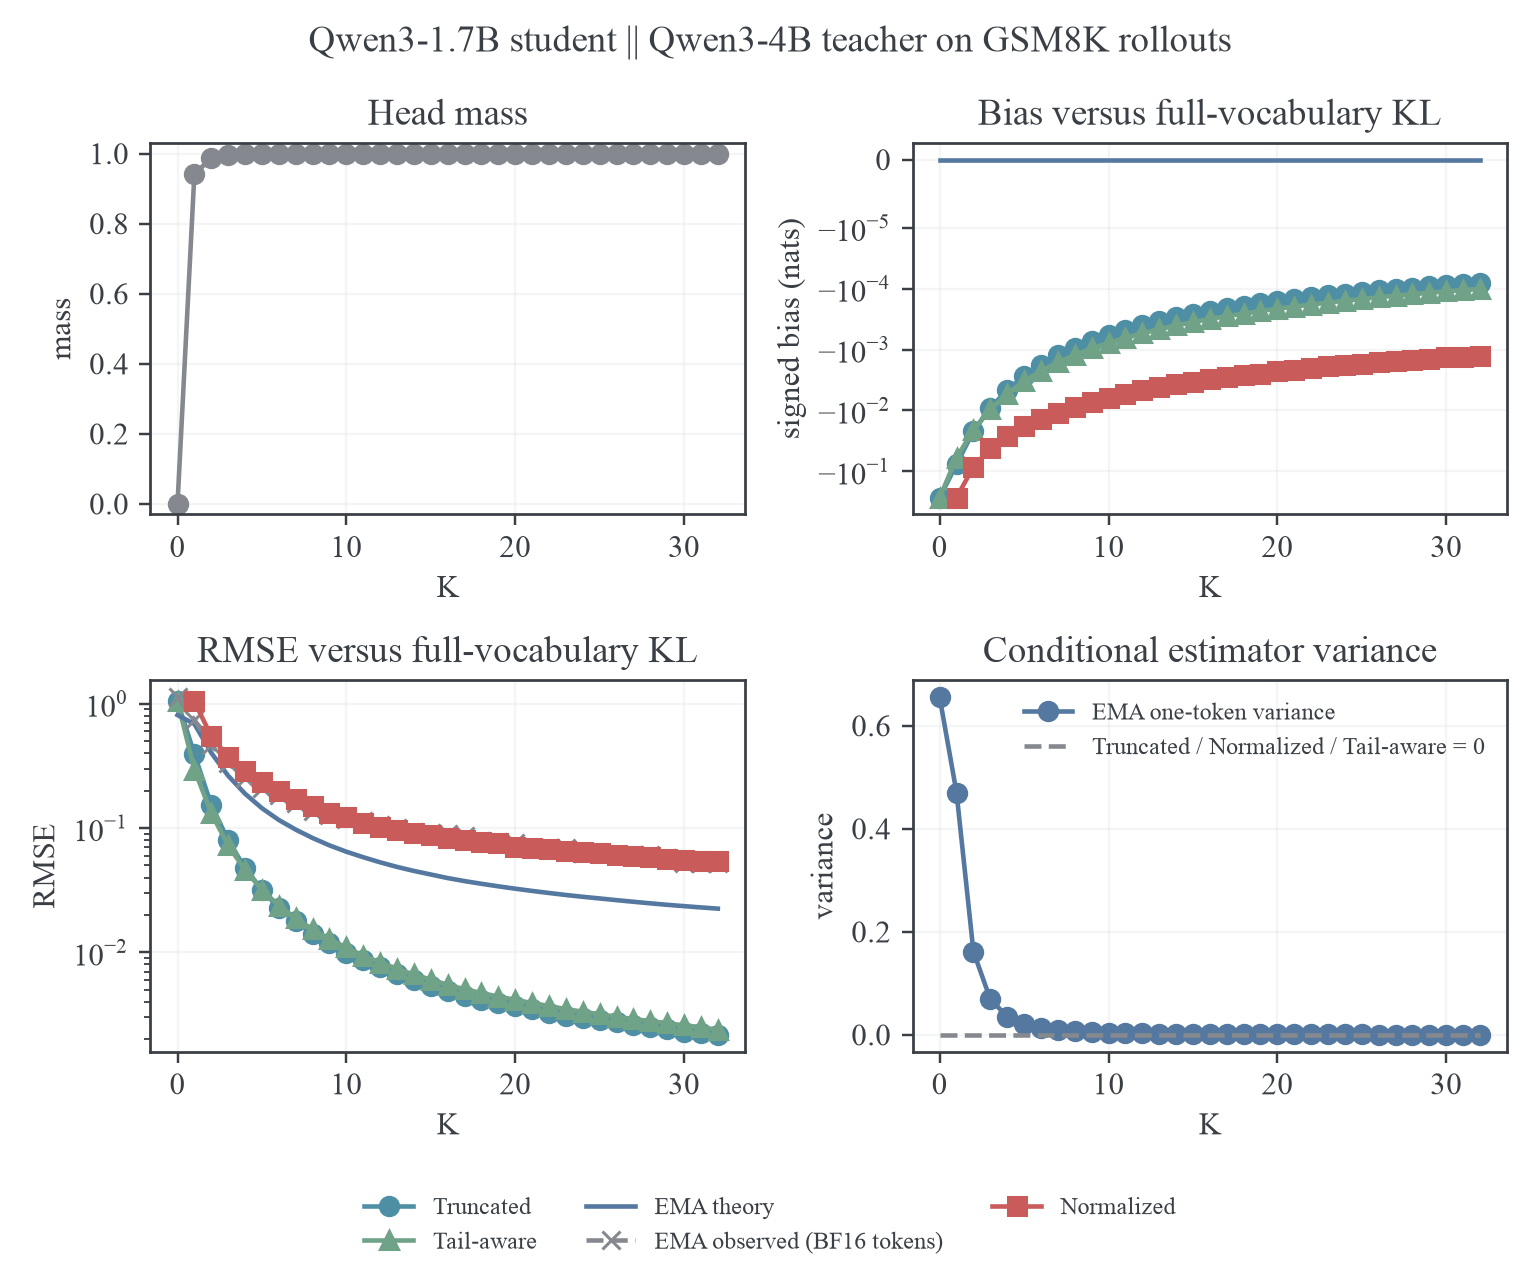
\includegraphics[width=0.96\textwidth]{../../results/qwen3_gsm8k_pair_kl/pair_kl_topk_metrics.png}
\caption{真实 GSM8K rollout 上四种 Top-$J$ KL 的误差曲线。bias 保留正负号；variance 是固定 prefix 的条件采样方差，不是不同 prefix 之间的数值方差。EMA observed 使用 bf16 rollout token，与 NF4 打分分布的理论曲线分开。}
\label{fig:qwen-topk-four}
\end{figure}

结果体现了四种定义之间的结构性差异。首先，student 的 top-$J$ 质量在 $J=4$ 时已经达到 $0.99747$，在 $J=32$ 时达到 $0.99996$，所以截断项的偏差和 RMSE 很快下降。其次，EMA Top-$J$ 在任何 $J$ 上都保持理论无偏，但只要尾部 log-ratio 的二阶矩仍然较大，sampled correction 就会带来明显方差；在 $J=32$ 时它的理论 RMSE 仍为 $0.02249$，高于截断项的 $0.00217$。这不是无偏性失效，而是典型的 bias--variance trade-off。

Normalized Top-$J$ 的行为不同。$J=1$ 时两边都是同一个 point mass，局部 KL 在数学上等于零，因此相对于完整 KL 的 bias 为 $-0.26932$。随着 $J$ 增大，条件分布逐渐包含更多质量，RMSE 从 $1.03968$ 降至 $0.05438$；但在 $J=32$ 时仍明显高于截断项。这说明归一化修复的是局部目标的概率尺度，而不是尾部 token-wise KL。它适合作为 dense local OPD 目标，却不能被解释为完整 KL 的高精度估计量。

Tail-Aware 的全量结果见表~\ref{tab:qwen-tail-aware}。其 RMSE 随 $J$ 单调下降，符合KL 估计章的支持集细化定理。在 $J=1,2,4$ 时，其 RMSE 小于 Truncated；在 $J=8,16,32$ 时，Truncated 略小。这正对应尾部质量项与尾部形状项的抵消：Tail-Aware 恢复质量项后，剩下的误差严格为非正的尾部形状偏差，而 Truncated 的两个遗漏项可以部分相互抵消。这个标量 RMSE 排序不等于训练稳定性的排序，也不能作为四种 OPD 训练方法最终性能的结论。

\begin{table}[ht]
\centering
\caption{同一批 350,166 个 prefix 上补全的 Tail-Aware 结果。条件采样方差在所有 $J$ 上均为零。}
\label{tab:qwen-tail-aware}
\begin{tabular}{rrrr}
\toprule
$J$ & mean Tail-Aware KL & bias & RMSE\\
\midrule
0 & 0 & -0.269321 & 1.039683\\
1 & 0.209759 & -0.059561 & 0.295078\\
2 & 0.248414 & -0.020907 & 0.131407\\
4 & 0.263978 & -0.005343 & 0.045886\\
8 & 0.268091 & -0.001230 & 0.015303\\
16 & 0.269006 & -0.000315 & 0.005493\\
32 & 0.269220 & -0.000101 & 0.002391\\
\bottomrule
\end{tabular}
\end{table}

这组实验不能支持“所有情况下都应该使用 normalized Top-$J$”这一结论。它支持更精确的选择规则：当我们需要在有限支持集上构造稳定的多 token 蒸馏 reward 时使用 $\mathcal K_J^{\mathrm{norm}}$；当我们需要完整 vanilla OPD KL 的估计时使用 EMA Top-$J$；当我们希望保留尾部总质量、又不承受 sampled correction 的方差时使用 Tail-Aware Top-$J$；Truncated Top-$J$ 则作为低方差、有明确尾部偏差的基线。
